% Options for packages loaded elsewhere
\PassOptionsToPackage{unicode}{hyperref}
\PassOptionsToPackage{hyphens}{url}
%
\documentclass[
]{book}
\usepackage{amsmath,amssymb}
\usepackage{lmodern}
\usepackage{iftex}
\ifPDFTeX
  \usepackage[T1]{fontenc}
  \usepackage[utf8]{inputenc}
  \usepackage{textcomp} % provide euro and other symbols
\else % if luatex or xetex
  \usepackage{unicode-math}
  \defaultfontfeatures{Scale=MatchLowercase}
  \defaultfontfeatures[\rmfamily]{Ligatures=TeX,Scale=1}
\fi
% Use upquote if available, for straight quotes in verbatim environments
\IfFileExists{upquote.sty}{\usepackage{upquote}}{}
\IfFileExists{microtype.sty}{% use microtype if available
  \usepackage[]{microtype}
  \UseMicrotypeSet[protrusion]{basicmath} % disable protrusion for tt fonts
}{}
\makeatletter
\@ifundefined{KOMAClassName}{% if non-KOMA class
  \IfFileExists{parskip.sty}{%
    \usepackage{parskip}
  }{% else
    \setlength{\parindent}{0pt}
    \setlength{\parskip}{6pt plus 2pt minus 1pt}}
}{% if KOMA class
  \KOMAoptions{parskip=half}}
\makeatother
\usepackage{xcolor}
\usepackage{color}
\usepackage{fancyvrb}
\newcommand{\VerbBar}{|}
\newcommand{\VERB}{\Verb[commandchars=\\\{\}]}
\DefineVerbatimEnvironment{Highlighting}{Verbatim}{commandchars=\\\{\}}
% Add ',fontsize=\small' for more characters per line
\usepackage{framed}
\definecolor{shadecolor}{RGB}{248,248,248}
\newenvironment{Shaded}{\begin{snugshade}}{\end{snugshade}}
\newcommand{\AlertTok}[1]{\textcolor[rgb]{0.94,0.16,0.16}{#1}}
\newcommand{\AnnotationTok}[1]{\textcolor[rgb]{0.56,0.35,0.01}{\textbf{\textit{#1}}}}
\newcommand{\AttributeTok}[1]{\textcolor[rgb]{0.77,0.63,0.00}{#1}}
\newcommand{\BaseNTok}[1]{\textcolor[rgb]{0.00,0.00,0.81}{#1}}
\newcommand{\BuiltInTok}[1]{#1}
\newcommand{\CharTok}[1]{\textcolor[rgb]{0.31,0.60,0.02}{#1}}
\newcommand{\CommentTok}[1]{\textcolor[rgb]{0.56,0.35,0.01}{\textit{#1}}}
\newcommand{\CommentVarTok}[1]{\textcolor[rgb]{0.56,0.35,0.01}{\textbf{\textit{#1}}}}
\newcommand{\ConstantTok}[1]{\textcolor[rgb]{0.00,0.00,0.00}{#1}}
\newcommand{\ControlFlowTok}[1]{\textcolor[rgb]{0.13,0.29,0.53}{\textbf{#1}}}
\newcommand{\DataTypeTok}[1]{\textcolor[rgb]{0.13,0.29,0.53}{#1}}
\newcommand{\DecValTok}[1]{\textcolor[rgb]{0.00,0.00,0.81}{#1}}
\newcommand{\DocumentationTok}[1]{\textcolor[rgb]{0.56,0.35,0.01}{\textbf{\textit{#1}}}}
\newcommand{\ErrorTok}[1]{\textcolor[rgb]{0.64,0.00,0.00}{\textbf{#1}}}
\newcommand{\ExtensionTok}[1]{#1}
\newcommand{\FloatTok}[1]{\textcolor[rgb]{0.00,0.00,0.81}{#1}}
\newcommand{\FunctionTok}[1]{\textcolor[rgb]{0.00,0.00,0.00}{#1}}
\newcommand{\ImportTok}[1]{#1}
\newcommand{\InformationTok}[1]{\textcolor[rgb]{0.56,0.35,0.01}{\textbf{\textit{#1}}}}
\newcommand{\KeywordTok}[1]{\textcolor[rgb]{0.13,0.29,0.53}{\textbf{#1}}}
\newcommand{\NormalTok}[1]{#1}
\newcommand{\OperatorTok}[1]{\textcolor[rgb]{0.81,0.36,0.00}{\textbf{#1}}}
\newcommand{\OtherTok}[1]{\textcolor[rgb]{0.56,0.35,0.01}{#1}}
\newcommand{\PreprocessorTok}[1]{\textcolor[rgb]{0.56,0.35,0.01}{\textit{#1}}}
\newcommand{\RegionMarkerTok}[1]{#1}
\newcommand{\SpecialCharTok}[1]{\textcolor[rgb]{0.00,0.00,0.00}{#1}}
\newcommand{\SpecialStringTok}[1]{\textcolor[rgb]{0.31,0.60,0.02}{#1}}
\newcommand{\StringTok}[1]{\textcolor[rgb]{0.31,0.60,0.02}{#1}}
\newcommand{\VariableTok}[1]{\textcolor[rgb]{0.00,0.00,0.00}{#1}}
\newcommand{\VerbatimStringTok}[1]{\textcolor[rgb]{0.31,0.60,0.02}{#1}}
\newcommand{\WarningTok}[1]{\textcolor[rgb]{0.56,0.35,0.01}{\textbf{\textit{#1}}}}
\usepackage{longtable,booktabs,array}
\usepackage{calc} % for calculating minipage widths
% Correct order of tables after \paragraph or \subparagraph
\usepackage{etoolbox}
\makeatletter
\patchcmd\longtable{\par}{\if@noskipsec\mbox{}\fi\par}{}{}
\makeatother
% Allow footnotes in longtable head/foot
\IfFileExists{footnotehyper.sty}{\usepackage{footnotehyper}}{\usepackage{footnote}}
\makesavenoteenv{longtable}
\usepackage{graphicx}
\makeatletter
\def\maxwidth{\ifdim\Gin@nat@width>\linewidth\linewidth\else\Gin@nat@width\fi}
\def\maxheight{\ifdim\Gin@nat@height>\textheight\textheight\else\Gin@nat@height\fi}
\makeatother
% Scale images if necessary, so that they will not overflow the page
% margins by default, and it is still possible to overwrite the defaults
% using explicit options in \includegraphics[width, height, ...]{}
\setkeys{Gin}{width=\maxwidth,height=\maxheight,keepaspectratio}
% Set default figure placement to htbp
\makeatletter
\def\fps@figure{htbp}
\makeatother
\setlength{\emergencystretch}{3em} % prevent overfull lines
\providecommand{\tightlist}{%
  \setlength{\itemsep}{0pt}\setlength{\parskip}{0pt}}
\setcounter{secnumdepth}{5}
\usepackage{booktabs}
\ifLuaTeX
  \usepackage{selnolig}  % disable illegal ligatures
\fi
\usepackage[]{natbib}
\bibliographystyle{plainnat}
\IfFileExists{bookmark.sty}{\usepackage{bookmark}}{\usepackage{hyperref}}
\IfFileExists{xurl.sty}{\usepackage{xurl}}{} % add URL line breaks if available
\urlstyle{same} % disable monospaced font for URLs
\hypersetup{
  pdftitle={TestWoodsmen},
  pdfauthor={Nayib Asis Elizalde},
  hidelinks,
  pdfcreator={LaTeX via pandoc}}

\title{TestWoodsmen}
\author{Nayib Asis Elizalde}
\date{7/14/2022}

\begin{document}
\maketitle

{
\setcounter{tocdepth}{1}
\tableofcontents
}
\hypertarget{intro}{%
\chapter{Intro}\label{intro}}

\textbf{MBAn Student's Guide to Ross and Ann Arbor}

\emph{\textasciitilde Live, Laugh, Ross\textasciitilde{}}

Situation and Proposed Solution:

As the first MBAn cohort, with almost every single one of us new to Ann Arbor and the Ross School of Business, we have faced challenges trying to adapt to a new environment. As a result, our group is seeking to help future generations of MBAn's by creating a detailed guide on Ross and an introduction to the uncontrollable world of business.

Our book will include different sections (listed below) explaining the transition to Ann Arbor, unspoken as well as established rules for navigating Ross, and other pieces of information that our team members have found useful in the last few weeks. We will accomplish this goal by following the principles outlined in our team charter.

\hypertarget{about-us}{%
\chapter{About us}\label{about-us}}

Get to know the Woodsmen, and what we're all about!

\hypertarget{who-is-tom-davis}{%
\section{Who is Tom Davis?}\label{who-is-tom-davis}}

\textbf{``Hello, World!''}

My Name is Tom Davis, I'm from Birmingham, MI, and I am a graduate student at the Ross School of Business working towards my Master of Business Analytics. I came to this program because I love \emph{music}. That might seem strange given we're not playing any instruments, but I think you'd be surprised how similar coding and chords can be.

Music, Business, and Software all require

\begin{itemize}
\tightlist
\item
  \emph{Creativity}
\item
  \emph{Problem Solving}
\item
  and \emph{Language Skills}
\end{itemize}

In addition, these three things are absolutely \textbf{fundamental} to our daily lives. We all utilize software, listen to music, and participate in the uncontrollable world of business every day. My end goal? Live at this intersection to help deliver listeners more of the music they love!

\includegraphics{https://i0.wp.com/haulixdaily.com/wp-content/uploads/2019/05/Music-Business-Success.jpg?w=1920\&ssl=1}

\hypertarget{who-is-alex-finci}{%
\section{Who is Alex Finci?}\label{who-is-alex-finci}}

My name is Alex Finci and I am a Master of Business Analytics student in the Ross School of Business at the University of Michigan. I have always been interested in the intersection of data and business and how companies use data analytics to gain insights into consumer behaviors to make business decision. And what better way to learn more about business analytics than through a Masters at Ross!

\textbf{Background}

I was born in Los Angeles, where I lived for the first ten years of my life. In 2006, my family moved just north of San Francisco, where my parents and older sister currently reside. I received my undergraduate degree at the University of Wisconsin-Madison, where I majored in Economics. I enjoy being active and playing sports, including basketball, tennis and golf. I am avid fan of Los Angeles' sports teams. I also like to hike and travel.

\begin{figure}

{\centering 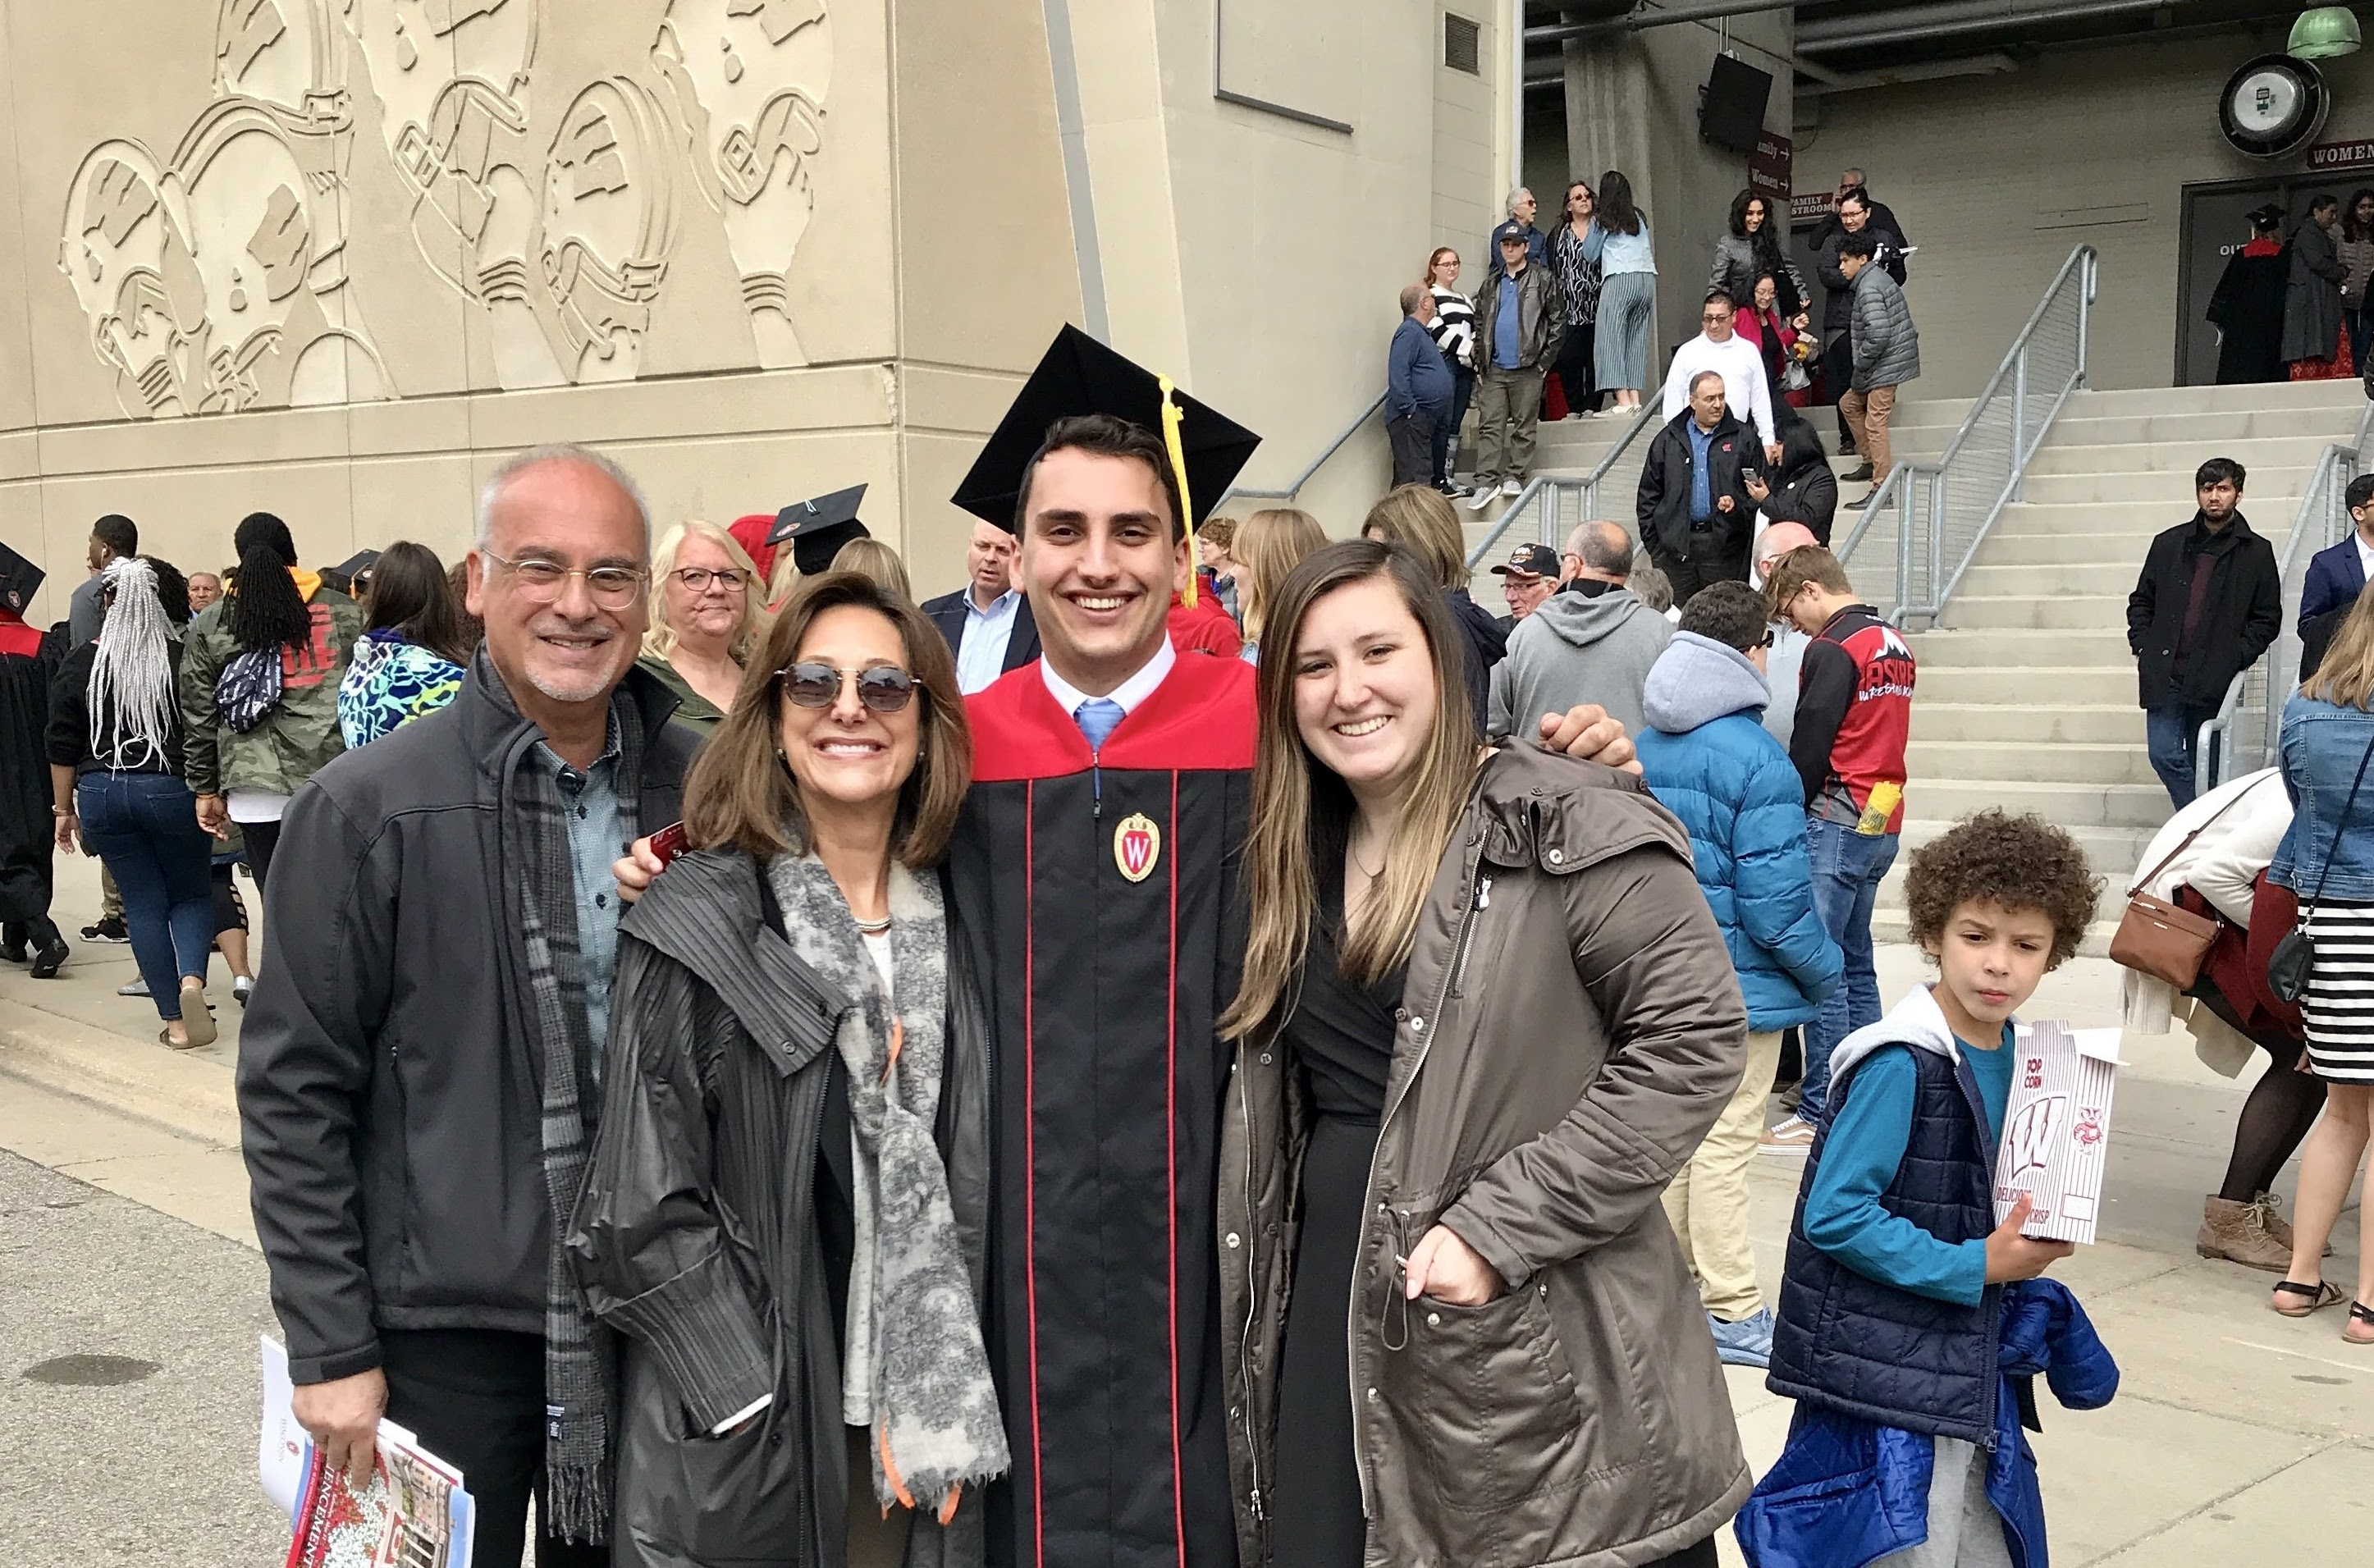
\includegraphics[width=0.8\linewidth]{IMG_4355} 

}

\end{figure}

\hypertarget{who-is-anthony-oliveri}{%
\section{Who is Anthony Oliveri?}\label{who-is-anthony-oliveri}}

I am from Long Island, New York and I currently live in Ann Arbor, Michigan as I am a Masters student at UM-Ann Arbor. I moved to Michigan in 2018 for my undergraduate education!

\begin{figure}
\centering
\includegraphics{https://media-exp1.licdn.com/dms/image/C5603AQGbQR9eOAFc9w/profile-displayphoto-shrink_400_400/0/1657558637851?e=1663200000\&v=beta\&t=Aqv-pWXUQxdrTJu1TT4ZM-Qo_b1ItTenlLsaFO-FHWs}
\caption{Me, 2022}
\end{figure}

\textbf{Credentials}

I graduated with a B.A. in Economics from Michigan in 2022 and now I am a Master of Business Analytics student at the University of Michigan - Ross School of Business. Go Blue!

\textbf{Goals}
I am passionate about data and I hope to learn how to contribute significant analyses in the future.

\textbf{Hobbies}

\begin{itemize}
\item
  All Sports! I watch Basketball, Baseball, and Football, but I will play almost any sport! My favorites to play are basketball, baseball, and volleyball.
\item
  Video Games
\item
  Hiking, Traveling, and Exploring
\end{itemize}

\textbf{Links}

\begin{itemize}
\item
  \href{https://www.linkedin.com/in/anthony-oliveri1/}{LinkedIn}
\item
  \href{https://www.facebook.com/anthony.oliveri.6/}{Facebook}
\item
  \href{https://www.instagram.com/aoliveri8/}{Instagram}
\end{itemize}

\hypertarget{who-is-nayib-asis-elizalde}{%
\section{Who is Nayib Asis Elizalde?}\label{who-is-nayib-asis-elizalde}}

I was born and raised in \emph{Monclova, Mexico}, where I lived with my parents and older sister until I turned 15. I then moved to the United States for school and have been here since (9th year)! I currently live in \emph{Ann Arbor, MI}.

I graduated from \emph{Dartmouth College} in 2020 (via Zoom) where I majored in Political Science focusing on Latin American politics. While there, I was part of different admissions and orientation groups, a Paganucci Fellow at the Tuck School of Business, and part of the executive board of my fraternity.

After college, I obtained my Master of Management with distinction from the \emph{Ross School of Business} at the \emph{University of Michigan}. I am currently pursuing a Master of Business Analytics also from Ross, and I served the program's student association as a Students Relations co-chair.

\textbf{Career Interests}

In the past, I have worked on different projects with Latin American companies seeking to tackle complex social issues through innovation. As a Paganucci Fellow working with Innova Schools in Peru and an intern at Dalberg Advisors doing consulting work in Mexico and Colombia, I learned about problem-solving, the role that businesses play in today's world, and how integrating new technology can lead to ground-breaking solutions.

In the future, I hope to pursue a career that allows me to have some sort of impact in the lives of others.

\textbf{Other Interests and Fun Facts}

\begin{itemize}
\item
  Going on runs (I am trying to run a half marathon this year)
\item
  Traveling to new places (really excited for for a trip to Florence this year)
\item
  Reading (I read 30 books in 2021)
\item
  Having fun with friends
\item
  My favorite quote: ``If you don't have a seat at the table, bring a folding chair.''
\end{itemize}

\hypertarget{who-is-runfan-yan}{%
\section{Who is Runfan Yan?}\label{who-is-runfan-yan}}

My name is Runfan Yan. I am from Ningbo, China and currently live in Ann Arbor as a master student in University of Michigan.

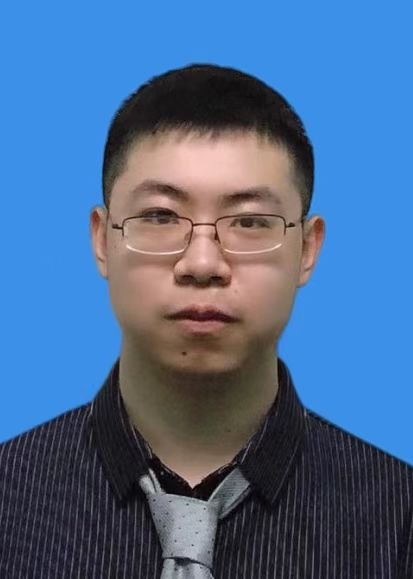
\includegraphics{Runfan_Photo.jpg}

\textbf{Personal Information}

\begin{itemize}
\item
  Mobile: 971-717-1702
\item
  Email: \href{mailto:runfanyan@gmail.com}{\nolinkurl{runfanyan@gmail.com}}
\end{itemize}

\textbf{Education Background}

University of Denver, BS in Business Administration, Major: Business Analytics, Minor: Mathematics, 09/2017 - 06/2021

University of Michigan, Master of Business Analytics, 06/2022 - 04/2023

\textbf{Internship Experience}

KPMG China, Tax Management Consulting Intern, 08/2021-11/2021

\begin{itemize}
\item
  Assisted to draft the solutions for incentive and tax consulting inquiry for clients and complied relevant materials
\item
  Responsible for solving client's problem of Tax e-Token update with repeated coordination with Tax Bureau, Bank of China, and KPMG departments; helped to identify the core issue and executed possible solutions
\item
  Reviewed clients' materials for the application of digitalization and intelligence demonstration; summarized the operation conditions to fulfill the requirement of declaration report
\end{itemize}

\textbf{Hobbies}

\begin{itemize}
\item
  Playing Badminton
\item
  Swimming
\item
  Reading
\item
  Traveling
\item
  Playing the piano
\end{itemize}

\textbf{Fun fact about me}

\begin{itemize}
\item
  I have been playing the piano since I was four years old
\item
  I once raised two parrots, but unfortunately they flew away inadvertently
\end{itemize}

\hypertarget{ross-administration}{%
\chapter{Ross Administration}\label{ross-administration}}

\hypertarget{buildings}{%
\section{Buildings}\label{buildings}}

\hypertarget{program-directors-deans-and-professors}{%
\section{Program Directors, Deans, and Professors}\label{program-directors-deans-and-professors}}

\hypertarget{places-to-study}{%
\chapter{Places to Study}\label{places-to-study}}

\hypertarget{booking-rooms}{%
\section{Booking Rooms}\label{booking-rooms}}

\hypertarget{interview-rooms}{%
\section{Interview Rooms}\label{interview-rooms}}

\hypertarget{libraries}{%
\section{Libraries}\label{libraries}}

\hypertarget{winter-garden}{%
\section{Winter Garden}\label{winter-garden}}

\textbf{MBAn Student's Guide to Ross and Ann Arbor}

\emph{\textasciitilde Live, Laugh, Ross\textasciitilde{}}

Situation and Proposed Solution:

As the first MBAn cohort, with almost every single one of us new to Ann Arbor and the Ross School of Business, we have faced challenges trying to adapt to a new environment. As a result, our group is seeking to help future generations of MBAn's by creating a detailed guide on Ross and an introduction to the uncontrollable world of business.

Our book will include different sections (listed below) explaining the transition to Ann Arbor, unspoken as well as established rules for navigating Ross, and other pieces of information that our team members have found useful in the last few weeks. We will accomplish this goal by following the principles outlined in our team charter.

Preliminary Table of Contents:

\begin{itemize}
\tightlist
\item
  Intro to Ross/MBAn
\item
  Ross administration

  \begin{itemize}
  \tightlist
  \item
    Buildings
  \item
    Program directors / deans / professors
  \end{itemize}
\item
  Places to Study

  \begin{itemize}
  \tightlist
  \item
    Booking rooms
  \item
    Interview rooms
  \item
    Libraries
  \item
    Winter Garden
  \end{itemize}
\item
  Ross Norms

  \begin{itemize}
  \tightlist
  \item
    Dress code

    \begin{itemize}
    \tightlist
    \item
      When to dress up, etc.
    \end{itemize}
  \item
    Timing of classes
  \end{itemize}
\item
  Classes and professors
\item
  Introduction to the CDO
\item
  Eating at Ross (restaurants that are within walking distance)
\item
  Important ross websites

  \begin{itemize}
  \tightlist
  \item
    Ross recruit, canvas, impact, handshake, my uofmhealth
  \end{itemize}
\item
  UHS / Health services

  \begin{itemize}
  \tightlist
  \item
    myuofmhealth
  \end{itemize}
\item
  Preparing for Group Projects and Presentations
\item
  Transportation

  \begin{itemize}
  \tightlist
  \item
    Busses, where to park, biking, preparing for the winter, etc.
  \end{itemize}
\end{itemize}

Areas to explore/further questions/Next steps:

\begin{itemize}
\tightlist
\item
  Interview fellow classmates as well as professors
\item
  Trying out new restaurants and establishments around Ross
\item
  Keep a journal where we write down our daily observations
\item
  Meet with MBAn 501 professors to ask further RMarkdown questions
\end{itemize}

\hypertarget{r-markdown}{%
\section{R Markdown}\label{r-markdown}}

\hypertarget{alex-finci-comment}{%
\section{Alex Finci Comment}\label{alex-finci-comment}}

\hypertarget{tom-davis-comment}{%
\section{Tom Davis Comment}\label{tom-davis-comment}}

\hypertarget{runfan-yan-comment}{%
\section{Runfan Yan Comment}\label{runfan-yan-comment}}

This is an R Markdown document. Markdown is a simple formatting syntax for authoring HTML, PDF, and MS Word documents. For more details on using R Markdown see \url{http://rmarkdown.rstudio.com}.

When you click the \textbf{Knit} button a document will be generated that includes both content as well as the output of any embedded R code chunks within the document. You can embed an R code chunk like this:

\begin{Shaded}
\begin{Highlighting}[]
\FunctionTok{summary}\NormalTok{(cars)}
\end{Highlighting}
\end{Shaded}

\begin{verbatim}
##      speed           dist       
##  Min.   : 4.0   Min.   :  2.00  
##  1st Qu.:12.0   1st Qu.: 26.00  
##  Median :15.0   Median : 36.00  
##  Mean   :15.4   Mean   : 42.98  
##  3rd Qu.:19.0   3rd Qu.: 56.00  
##  Max.   :25.0   Max.   :120.00
\end{verbatim}

\hypertarget{including-plots}{%
\section{Including Plots}\label{including-plots}}

You can also embed plots, for example:

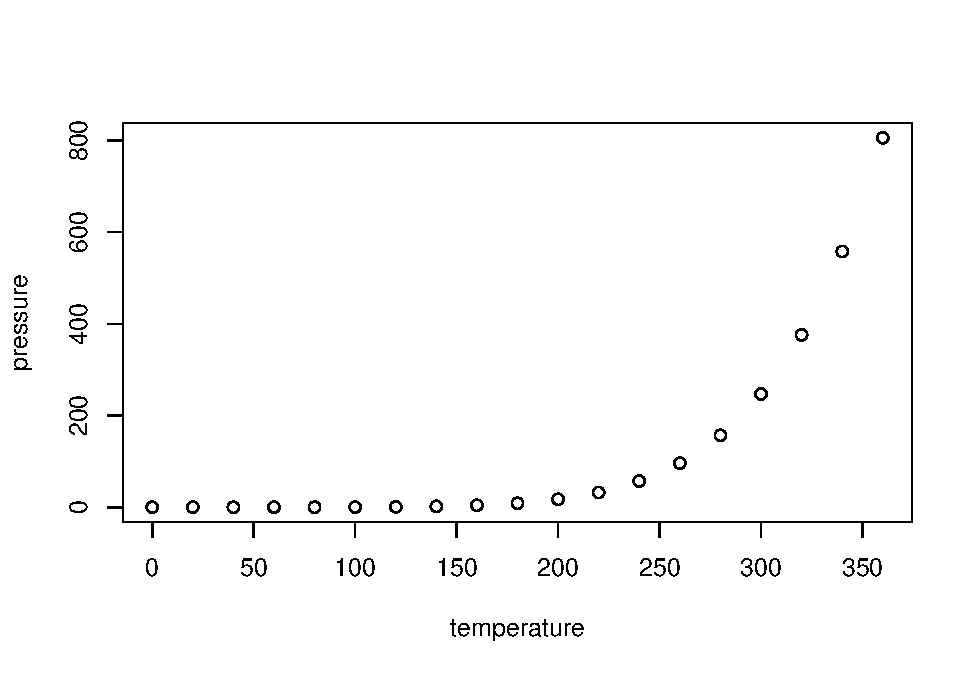
\includegraphics{_main_files/figure-latex/pressure-1.pdf}

Note that the \texttt{echo\ =\ FALSE} parameter was added to the code chunk to prevent printing of the R code that generated the plot.

  \bibliography{book.bib,packages.bib}

\end{document}
